\chapter{Automatic Software Diversification for WebAssembly}
\label{tech}

This dissertation makes contributions to the field of Software Diversification for \Wasm with three main technical contributions: CROW, MEWE, and wasm-mutate.
In the following text we detail each one of these contributions.

%\todo{Start here. 4 pages each and 2 pages discussion. Target 20 pages.}

\msection{Generating Software Diversification for WebAssembly}

\Wasm programs are obtained ahead of time.
This means that the source code is compiled to \wasm binaries before they come to host engines to be compiled to machine code and then executed.
The process of obtaining a \Wasm program can be roughly separated in three high-level components: source code, compiler and the generated \Wasm program.
Software Diversification can be applied to any of these three main components.
Yet, applying diversification at the source code level is not practical since it will limit such approach to specific programming languages, e.g. one diversifier per possible language compiling to \Wasm.
Therefore, this thesis focus on the other two components, the compiler and the generated \Wasm program itself.
In \autoref{fig:approach_landscape} we show the landscape of our approaches.
They focus on two main strategies: compiler-based and binary-based.
The compiler-based approaches are highlighted in red and green, while the binary-based approaches are highlighted in blue.

% Compiler based approaches
Our compiler-based approaches are illustrated in \autoref{fig:approach_landscape} as the red  and green squared tooling.
The work of Hilbig et al. \cite{Hilbig2021AnES} in 2021 highlights that 70\% of the \wasm\ binaries in the wild are created with LLVM-based compilers. 
Based on such analysis, we provide artificial software diversity for \wasm\ as a compiler-based approach through LLVM.
LLVM is a compound of three main components \cite{llvmofficialweb}. 
First, the frontend (compilers such as clang and rustc) converts the program source code to LLVM intermediate representation (LLVM IR). 
Second, optimization and transformation processes improve the LLVM IR. 
Third and final, the backend component is in charge of generating the target Instruction Set.
We alter the LLVM pipeline that compiles source code to Wasm by introducing a diversifier component.  
The diversifier generates LLVM IR variants from the output of the frontend. 
The diversifier and the custom Wasm LLVM backend compose CROW, which creates \wasm program variants out of a source code program. 
In addition, an orthogonal tool comes from the generation of LLVM IR variants, MEWE \cite{MEWE}, which merges and creates multivariant binaries to provide Multivariant Execution for \wasm.  

\begin{figure}[h]
	\centering
	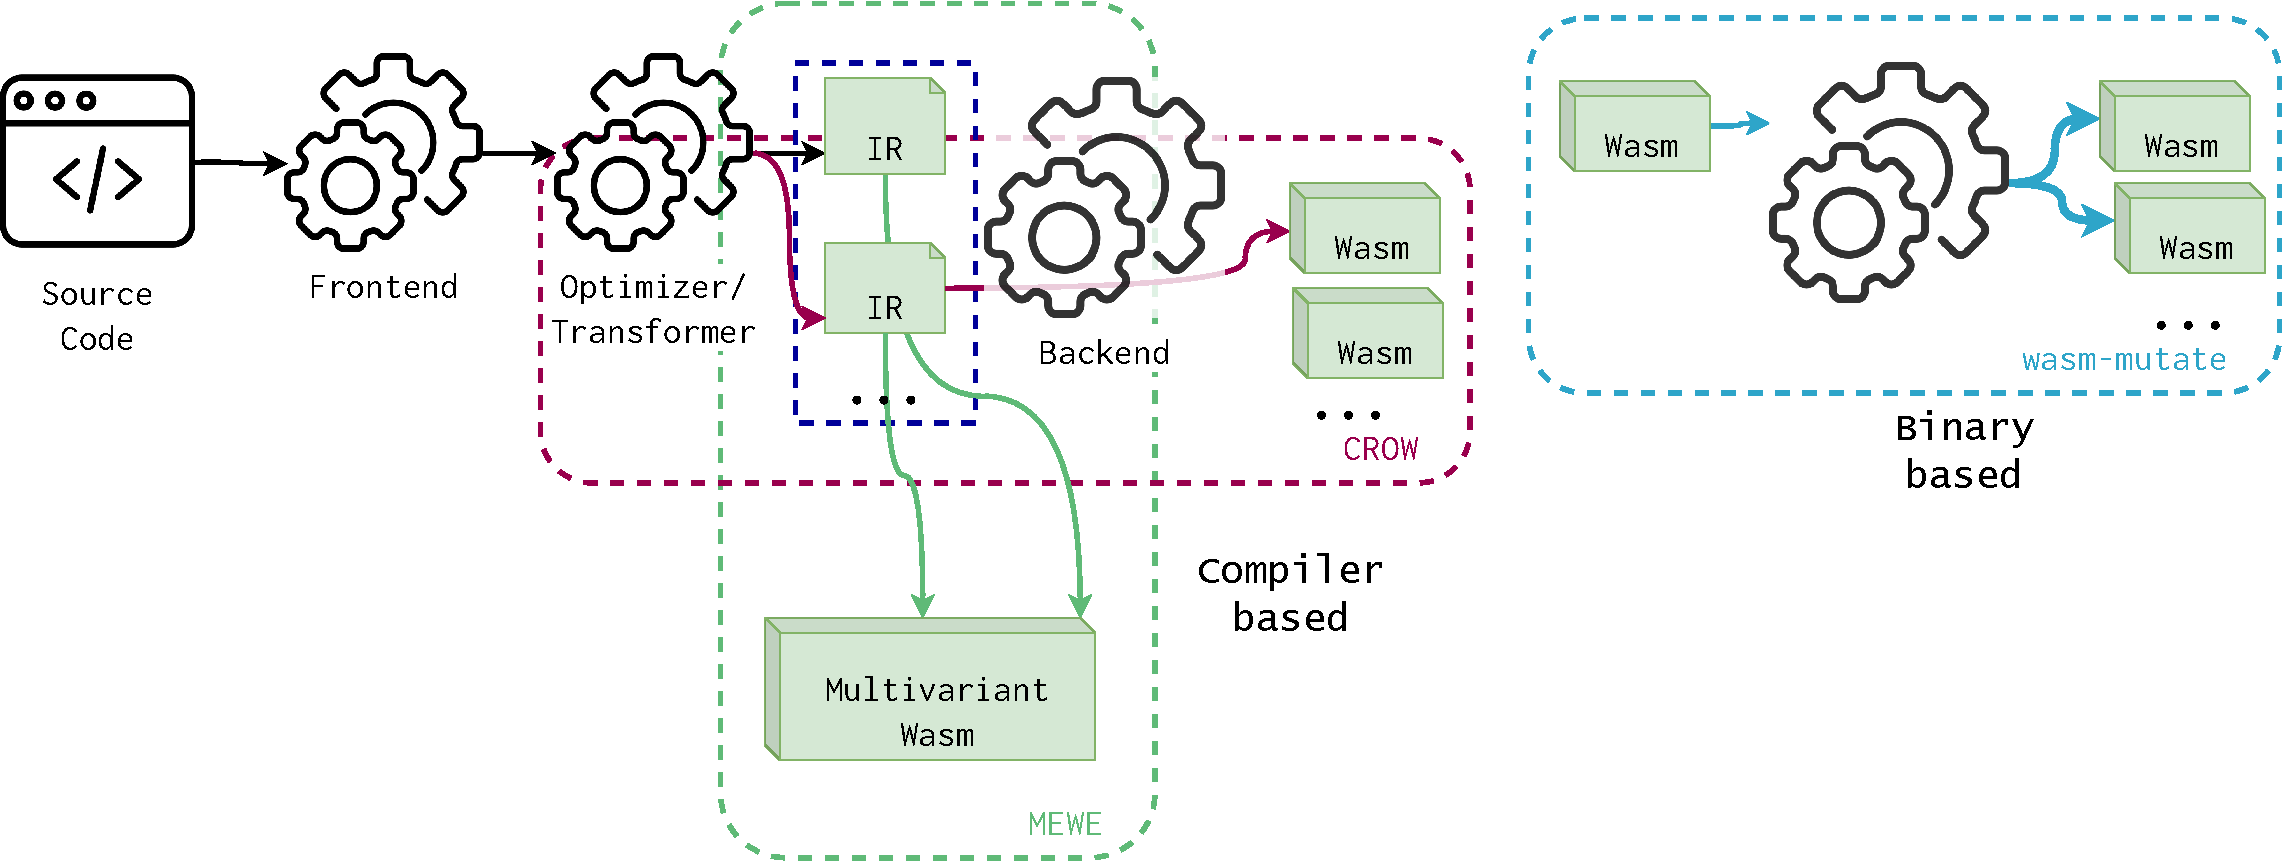
\includegraphics[width=1.0\textwidth]{figures/landscape.pdf}
	\caption{Approach landscape.}
	\label{fig:approach_landscape}
\end{figure}



% Move the following
%Other solutions would have been to diversify at the source-code level or the \wasm\ binary level. However, these facts would limit the applicability of our work.
%Our approach is more general as diversification also will work for other LLVM backends.





\msection{CROW: Code Randomization of WebAssembly}
\label{section:crow}

% Overview
This section describes the red squared tooling in \autoref{fig:approach_landscape} named CROW  \cite{CROW}. 
CROW is a tool tailored to create semantically equivalent \wasm\ variants from an LLVM front-end output.
Using a custom Wasm LLVM backend, it generates the Wasm binary variants.


In \autoref{diagrams:crow}, we describe the workflow of CROW to create program variants.
The Diversifier in CROW is composed by two main processes, \textit{exploration} and \textit{combining}. 
The \emph{exploration} process operates at the instruction level for each function in its input LLVM.
For all LLVM instructions, CROW produces a collection of functionally equivalent code replacements.   
In the \emph{combining} stage, CROW assembles the code replacements to generate different LLVM IR variants.
CROW generates the LLVM IR variants by traversing the power set of all possible combinations of code replacements.
Finally, the custom Wasm LLVM backend compiles the assembled LLVM IR variants into \wasm\ binaries.
In the following text, we describe our design decisions. 
%All our implementation choices are based on one premise: \emph{each design decision should increase the number of \wasm\ variants that CROW creates.}
%\subsection*{Overview}

\begin{figure*}[h]
    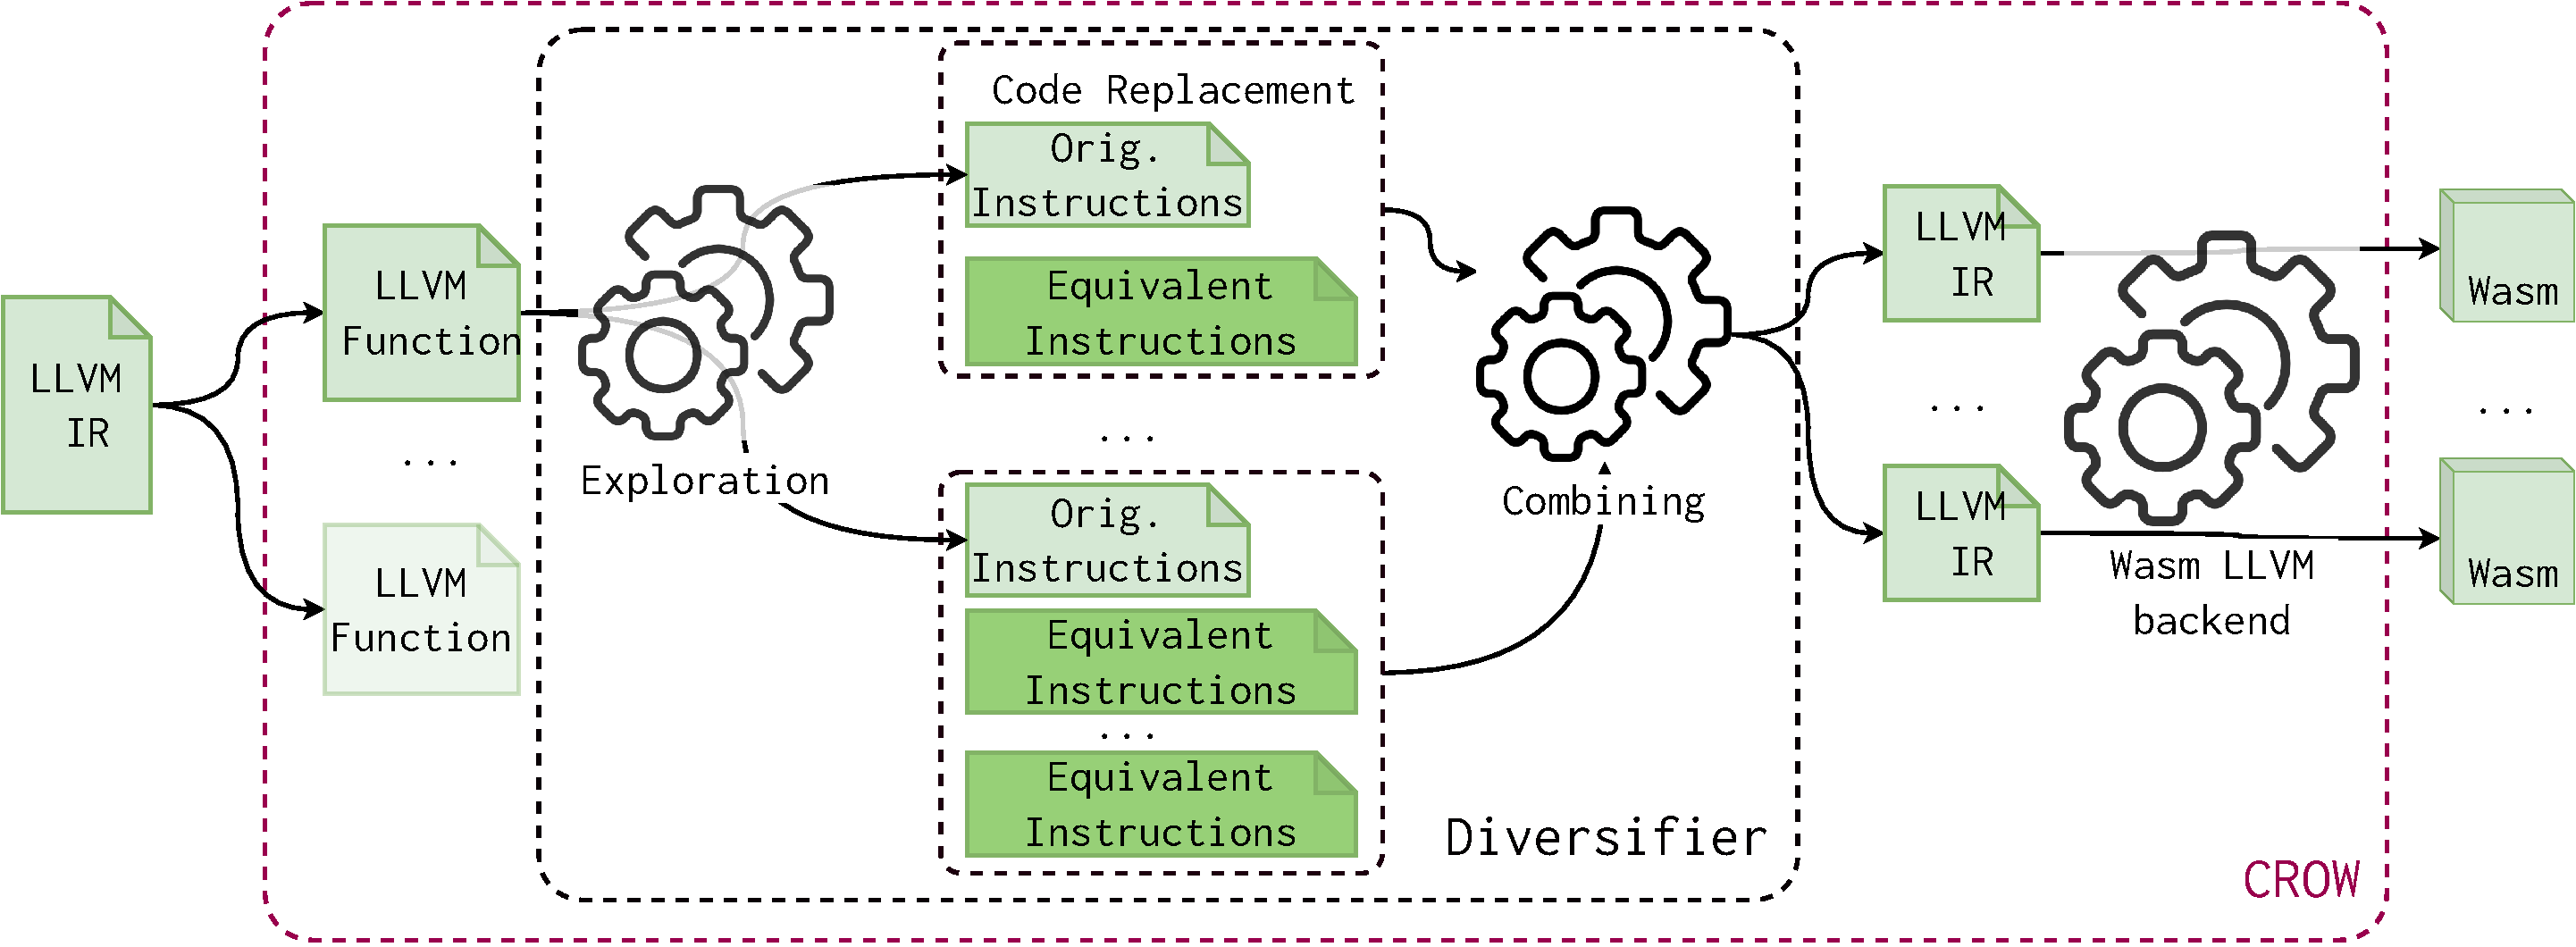
\includegraphics[width=\linewidth]{diagrams/generation/crow.drawio.pdf}
    \caption{CROW components following the diagram in \autoref{diagrams:generic}. CROW takes LLVM IR to generate functionally equivalent code replacements. Then, CROW assembles program variants by combining them.}
    \label{diagrams:crow}
\end{figure*}


%CROW operates at the code block level, taking them from the functions defined inside the input LLVM bitcode module. 
%In addition, the retargeted superoptimizer is in charge of finding the potential places in the original code blocks where a replacement can be applied. Finally, we use the enumerative synthesis strategy of the retargeted superoptimizer to generate code replacements.
%The code replacements generated through synthesis are verified, according to \autoref{def:functional-equivalence}, by internally using a theorem prover. 

%\emph{Exploration}
\msubsection{Variants' generation}

The primary component of CROW's exploration process is its code replacements generation strategy. The diversifier implemented in CROW is based on the proposed superdiversifier of Jacob \etal \cite{jacob2008superdiversifier}.
A superoptimizer focuses on \emph{searching} for a new program that is faster or smaller than the original code while preserving its functionality.
The concept of superoptimizing a program dates back to 1987, with the seminal work of Massalin \cite{Massalin1987} which proposes an exhaustive exploration of the solution space. The search space is defined by choosing a subset of the machine's instruction set and generating combinations of optimized programs, sorted by code size in ascending order. If any of these programs is found to perform the same function as the source program, the search halts. On the contrary, a superdiversifier keeps all intermediate search results despite their performance. 

% Why and main change
We use the superdiversifier idea of Jacob and colleagues to implement CROW because of two main reasons.
First, the code replacements generated by this technique outperform diversification strategies based on handwritten rules \todo{This is contradictory to our binary solution.}. 
Concretely, we can control the quality of the generated codes. 
Besides, CROW always generates equivalent programs because it is based on a solver to check for equivalence. 
Second, there is a battle-tested superoptimizer for LLVM, Souper \cite{Sasnauskas2017Souper:Superoptimizer}. 
This latter makes it feasible the construction of a generic LLVM superdiversifier. 

% This paragraph is hard to read
% How Souper works and why we can modify if
% Souper works as follows.
We modify Souper to keep all possible solutions in their searching algorithm.
Souper builds a Data Flow Graph for each LLVM integer-returning instruction. 
Then, for each Data Flow Graph, Souper exhaustively builds all possible expressions from a subset of the LLVM IR language.
Each syntactically correct expression in the search space is semantically checked versus the original with a theorem solver. Souper synthesizes the replacements in increasing size. Thus, the first found equivalent transformation is the optimal replacement result of the searching. 
CROW keeps more equivalent replacements during the searching by removing the halting criteria. Instead the original halting conditions, CROW does not halt when it finds the first replacement. CROW continues the search until a timeout is reached or the replacements grow to a size larger that a predefined threshold. 

Notice that the searching space increases exponentially with the size of the LLVM IR language subset. Thus,
we prevent Souper from synthesizing instructions with no correspondence in the \wasm\ backend. This decision reduces the searching space. For example, creating an expression having the  \texttt{freeze} LLVM instructions will increase the searching space for instruction without a Wasm's opcode in the end.
Moreover, we disable the majority of the pruning strategies of Souper for the sake of more program variants.
For example, Souper prevents the generation of the commutative operations during the searching.
On the contrary, CROW still uses such transformation as a strategy to generate program variants. 

\msubsection{Constant inferring}

One of the code transformation strategies of Souper does \emph{constant inferring}. This means that Souper infers pieces of code as a single constant assignment. In particular, Souper focuses on variables that are used to control branches.
By extending Souper as a superdiversifier, we add this transformation strategy as a new mutation strategy to the ones defined in \autoref{sota:sota}. 


After a \emph{constant inferring}, the generated program is considerably different from the original program, being suitable for diversification.
Let us illustrate the case with an example.
The Babbage problem code in \autoref{babbage} is composed of a loop that stops when it discovers the smaller number that fits with the Babbage condition in Line 4.


{


\begin{minipage}[t]{0.47\linewidth}
        \lstset{
        language=C,
        style=CStyle,
        columns=fullflexible,
        breaklines=true,
        belowcaptionskip=30pt,
        abovecaptionskip=1pt,
        columns=fullflexible,
        breaklines=true, 
        caption={Babbage problem.},
        label=babbage,
        postbreak=\mbox{\textcolor{red}{$\hookrightarrow$}\space}
    } 
    \begin{lstlisting}[numbers=left]
    int babbage() {
        int current = 0,
            square;
        while ((square=current*current) % 1000000 != 269696) {
            current++;
        }
        printf ("The number is %d\n", current);
        return 0 ;
    }
    \end{lstlisting}
\end{minipage}
\begin{minipage}[t]{0.48\linewidth}
        \lstset{
        language=C,
        style=CStyle,
        columns=fullflexible,
        breaklines=true,
        belowcaptionskip=3pt,
        abovecaptionskip=1pt,
        columns=fullflexible,
        breaklines=true, 
        caption={Constant inferring transformation over the original Babbage problem in \autoref{babbage}.},
        label=inferring,
        postbreak=\mbox{\textcolor{red}{$\hookrightarrow$}\space}
    } 
    \begin{lstlisting}[]
int babbage() {
    @int current = 25264;@
    
    


    printf ("The number is %d\n", current);
    return 0 ;
}
    \end{lstlisting}
\end{minipage}
}
% llvm-opt: rool unroll
In theory, this value can also be inferred by unrolling the loop the correct number of times with the LLVM toolchain.
However, standard LLVM tools cannot unroll the \texttt{\textbf{while}}-loop because the loop count is too large.
% Souper
The original Souper deals with this case, generating the program in \autoref{inferring}. It infers the value of \texttt{current} in Line 2 such that the Babbage condition is reached. Therefore, the condition in the loop will always be false. Then, the loop is dead code and is removed in the final compilation. 
The new program in \autoref{inferring} is remarkably smaller and faster than the original code. Therefore, it offers differences both statically and at runtime\footnote{ Notice that for the sake of illustration, we show both codes in C language, this process inside CROW is performed directly in LLVM IR. Also, notice that the two programs in the example follow the definition of \emph{functional equivalence} discussed in \autoref{sota:sota}.}.




%\subsection{Removing subsequent optimizations for LLVM}

During the implementation of CROW, we have the premise of removing all built-in optimizations in the LLVM backend that could reverse Wasm variants.
Therefore, we modify the \wasm\ backend.
We disable all optimizations in the \wasm\ backend that could reverse the CROW transformations.
In the following enumeration, we list three concrete optimizations that we remove from the \wasm~backend.\footnote{
We only illustrate three of the removed optimization for the sake of simplicity.}

\begin{itemize}
    \item Constant folding: this optimization calculates the operation over two (or more) constants in compiling time, and replaces the original expression by its constant result. For example, let us suppose \texttt{$a = 10 + 12$} a subexpression to be compiled, with the original optimization, the \wasm~ backend replaces it by \texttt{$a = 22$}.
    
    \item Expressions normalization: in this case, the comparison operations are normalized to its complementary operation, e.g. \texttt{$a > b$} is always replaced by \texttt{$b <= a$}.
    
    \item Redundant operation removal: expressions such as the multiplication of variables by \texttt{$a = b2^n$} are replaced by shift left operations \texttt{$a = b << n$}.  
\end{itemize}


\msubsection{CROW instantiation}
\label{section:crow:example}
%In \autoref{section:crow} we describe the main components and contributions of CROW. In this section we instantiate the workflow presented in \autoref{workflow} from the input of an example C code to the generation of a pool of \wasm\ program variants.

Let us illustrate how CROW works with the simple example code in \autoref{CExample}. The \texttt{f} function calculates the value of $2 * x + x$ where \texttt{x} is the input for the function.  CROW compiles this source code and generates the intermediate LLVM bitcode in the left most part of \autoref{example:crow:original:llvm}. CROW potentially finds two integer returning instructions to look for variants, as the right-most part of \autoref{example:crow:original:llvm} shows.

% snippet of code showing the detection of code blocks
%\begin{minipage}[t]{.9\linewidth}
%\begin{code}
    \lstset{
        language=C,
        basicstyle=\small\ttfamily,captionpos=b,caption={C function that calculates the quantity $2x + x$.},label=CExample, frame=b}
    
    \begin{lstlisting}[style=CStyle]
int f(int x) { 
    return 2 * x + x; 
}    
    \end{lstlisting}
%\end{code}
\end{minipage}

\lstdefinelanguage{LLVM}
    {morekeywords={i32,mul,align,nsw,add,load,store,define,br, ret, shl, ret},
    sensitive=false,
    morecomment=[l]{;},
    morecomment=[s]{;}{;},
    morestring=[b],
}

\lstdefinestyle{nccode}{
    numbers=left,
    tabsize=4,
    showspaces=false,
    breaklines=true, 
    showstringspaces=false,
    moredelim=**[is][{\btHL[fill=black!10]}]{`}{`},
    moredelim=**[is][{\btHL[fill=celadon!40]}]{!}{!}
}
\lstset{
    language=LLVM,
    style=nccode,
    %basicstyle=\small\ttfamily,
    columns=fullflexible,
    breaklines=true
}

\begin{minipage}[t]{0.9\linewidth}
    
    \lstset{numbers=none}
    \noindent\begin{minipage}[t]{.34\linewidth}
    \centering
    \begin{lstlisting}[xleftmargin=1em,escapechar=?]
    define i32 @f(i32) {

      %2 = mul nsw i32 %0,2
      %3 = add nsw i32 %0,%2 

      ret i32 %3
    }
    
    define i32 @main() {
      %1 = tail call i32 @f(i32 10)
      ret i32 %1
    }
    \end{lstlisting}
    \end{minipage}%\hfill%
    \begin{minipage}[t]{.32\linewidth}
        \begin{lstlisting}[xleftmargin=1em,escapechar=?]
?Replacement candidates for code\_1?

`%2 = mul nsw i32 %0,2`

!%2 = add nsw i32 %0,%0!

!%2 = shl nsw i32 %0, 1:i32!
    \end{lstlisting}
    \end{minipage}%\hfill%
    \begin{minipage}[t]{.32\linewidth}
        \lstdefinestyle{nccode}{
        tabsize=4, 
        showspaces=false,
        breaklines=true, 
        showstringspaces=false,
        moredelim=**[is][{\btHL[fill=black!10]}]{`}{`},
        moredelim=**[is][{\btHL[fill=celadon!40]}]{!}{!}
        }
        \lstset{
            language=LLVM,
            style=nccode,
            columns=fullflexible,
            breaklines=true,
            belowcaptionskip=1pt,
            abovecaptionskip=1pt,
        } 
        \begin{lstlisting}[name={B},escapechar=?]
?Replacement candidates for code\_2?

`%3 = add nsw i32 %0,%2`

!%3 = mul nsw %0, 3:i32!
        \end{lstlisting}
    \end{minipage}
    \centering
    \hrule
    \vspace{2mm}
    \captionof{lstlisting}{LLVM's intermediate representation program, its extracted instructions and replacement candidates. Gray highlighted lines represent original code, green for code replacements. }\label{example:crow:original:llvm}
\end{minipage}

\begin{minipage}[t]{.9\linewidth}
    \lstset{numbers=none}
    \noindent\begin{minipage}[t]{.5\linewidth}
    \begin{lstlisting}[xleftmargin=1em,escapechar=?]
`%2 = mul nsw i32 %0,2`
`%3 = add nsw i32 %0,%2`

!%2 = add nsw i32 %0,%0!
`%3 = add nsw i32 %0,%2`

!%2 = shl nsw i32 %0, 1:i32!
`%3 = add nsw i32 %0,%2`

    \end{lstlisting}
    \end{minipage}%\hfill%
    \begin{minipage}[t]{.5\linewidth}
        \lstdefinestyle{nccode}{
        tabsize=4, 
        showspaces=false,
        breaklines=true, 
        showstringspaces=false,
        moredelim=**[is][{\btHL[fill=black!10]}]{`}{`},
        moredelim=**[is][{\btHL[fill=celadon!40]}]{!}{!},
        moredelim=**[is][{\btHL[fill=weborange!40]}]{'}{'}
        }
        \lstset{
            language=LLVM,
            style=nccode,
            columns=fullflexible,
            breaklines=true,
            belowcaptionskip=1pt,
            abovecaptionskip=1pt,
        } 
        \begin{lstlisting}[xleftmargin=1em,escapechar=?]
'%2 = mul nsw i32 %0,2'
!%3 = mul nsw %0, 3:i32!

'%2 = add nsw i32 %0,%0'
!%3 = mul nsw %0, 3:i32!

'%2 = shl nsw i32 %0, 1:i32'
!%3 = mul nsw %0, 3:i32!

    \end{lstlisting}
    \end{minipage}
    \centering
    \hrule
    \vspace{2mm}
    \captionof{lstlisting}{Candidate code replacements combination. Orange highlighted code illustrate replacement candidate overlapping.}\label{example:crow:original:combination}
\end{minipage}


    

CROW, detects \texttt{code\_1} and \texttt{code\_2} as the enclosing boxes in the left most part of \autoref{example:crow:original:llvm} shows. CROW synthesizes $2 + 1$ candidate code replacements for each code respectively as the green highlighted lines show in the right most parts of \autoref{example:crow:original:llvm}.
The baseline strategy of CROW is to generate variants out of all possible combinations of the candidate code replacements, \ie uses the power set of all candidate code replacements.

In the example, the power set is the cartesian product of the found candidate code replacements for each code block, including the original ones, as \autoref{example:crow:original:combination} shows. The power set size results in $6$ potential function variants. Yet, the generation stage would eventually generate $4$ variants from the original program. CROW generated 4 statically different Wasm  files, as \autoref{example:crow:variants:wasm} illustrates. This gap between the potential and the actual number of variants is a consequence of the redundancy among the bitcode variants when composed into one. In other words, if the replaced code removes other code blocks, all possible combinations having it will be in the end the same program. In the example case, replacing \texttt{code\_2} by \texttt{mul nsw \%0, 3}, turns \texttt{code\_1} into dead code, thus, later replacements generate the same program variants. The rightmost part of \autoref{example:crow:original:combination} illustrates how for three different combinations, CROW produces the same variant. We call this phenomenon a \emph{code replacement overlapping}{Software!Replacement overlapping}.

%\lstdefinestyle{nccode}{
        numbers=none,
        firstnumber=2,
        stepnumber=1,
        numbersep=10pt,
        tabsize=4, 
        showspaces=false,
        breaklines=true, 
        showstringspaces=false,
    moredelim=**[is][\btHL]{`}{`},
    moredelim=**[is][{\btHL[fill=black!10]}]{`}{`},
    moredelim=**[is][{\btHL[fill=celadon!40]}]{!}{!}
}

\lstset{
    language=WAT,
    style=nccode,
    basicstyle=\footnotesize\ttfamily,
    columns=fullflexible,
    breaklines=true
}


\begin{minipage}[t]{0.9\linewidth}
    \lstset{numbers=none}
    \noindent\begin{minipage}[t]{.45\linewidth}
    \begin{lstlisting}[xleftmargin=1em,escapechar=?]
func $f (param i32) (result i32)
   local.get 0
    `i32.const 2`
    `i32.mul`
    `local.get 0`
    `i32.add`

        \end{lstlisting}
\begin{lstlisting}[xleftmargin=1em,escapechar=?]
func $f (param i32) (result i32)
    local.get 0
    !local.get 0!
    !i32.add!
    `local.get 0`
    `i32.add`

                \end{lstlisting}
    \end{minipage}\hfill
    \noindent\begin{minipage}[t]{.45\linewidth}
\begin{lstlisting}[xleftmargin=1em,escapechar=?]
func $f (param i32) (result i32)
    local.get 0
    !i32.const 1!
    !i32.shl!
    `local.get 0`
    `i32.add`

    \end{lstlisting}
\begin{lstlisting}[xleftmargin=1em,escapechar=?]
func $f (param i32) (result i32)
    local.get 0
    !i32.const 3!
    !i32.mul!

        \end{lstlisting}
    \end{minipage}

    \centering
    \hrule
    \vspace{2mm}
    \captionof{lstlisting}{Wasm  program variants generated from program \autoref{CExample}.}\label{example:crow:variants:wasm}
\end{minipage}




One might think that a reasonable heuristic could be implemented to avoid such overlapping cases. Instead, we have found it easier and faster to generate the variants with the combination of the replacement and check their uniqueness after the program variant is compiled. This prevents us from having an expensive checking for overlapping inside the CROW code. Still, this phenomenon calls for later optimizations in future works.


%\subsection{Combining replacements}

When we retarget Souper, to create variants, we recombine all code replacements, including those for which a constant inferring was performed.
This allows us to create variants that are also better than the original program in terms of size and performance. Most of the Artificial Software Diversification  works generate variants that are as performant or iller than the original program. By using a superdiversifier, we could be able to generate variants that are better, in terms of performance, than the original program. This will give the option to developers to decide between performance and diversification without sacrificing the former. 

On the other hand, when Souper finds a replacement, it is applied to all equal instructions in the original LLVM binary. In our implementation, we apply the transformation only to the instruction for which it was found in the first place. For example, if we find a replacement that is suitable for $N$ difference places in the original program, we generate $N$ different programs by applying the transformation in only one place at a time. Notice that this strategy provides a combinatorial explosion of program variants as soon as the number of replacements increases.



\msection{MEWE: Multi-variant Execution for WebAssembly}
\label{section:mewe}

\renewcommand{\tool}{MEWE\xspace}
% Overview
This section describes MEWE \cite{MEWE}. 
\tool synthesizes diversified function variants by using CROW.
It then provides execution-path randomization in a Multivariant Execution (MVE).
The tool generates application-level multivariant binaries without changing the operating system or \wasm\ runtime.
MEWE creates an MVE by intermixing functions for which CROW generates variants, as step \step{2} in \autoref{diagrams:generic} shows.
CROW generates each one of these variants with fine-grained diversification at the instruction level, applying the majority of the strategies discussed in \autoref{sota:sota} and \emph{constant inferring}. \tool adds a new mutation strategy. It inlines function variants when appropriate, resulting in call stack diversification at runtime.

In \autoref{workflow} we zoom MEWE from the blue highlighted square in \autoref{diagrams:generic}. MEWE takes the LLVM IR variants generated by CROW's diversifier. It then merges LLVM IR variants into a Wasm multivariant.
In the figure, we highlight the two components of MEWE, \emph{Multivariant Generation} and the \emph{Mixer}.
In the \emph{Multivariant Generation} process, 
MEWE merges the LLVM IR variants created by CROW and creates an LLVM multivariant binary.
The merging of the variants intermixes the calling of function variants, allowing the execution path randomization.

\emph{The Mixer} augments the LLVM multivariant binary with a random generator. The random generator is needed to perform the execution-path randomization.
Also, \emph{The Mixer} fixes the entrypoint in the multivariant binary.
Finally, MEWE generates a standalone multivariant \wasm\ binary using the same custom Wasm LLVM backend from CROW.
Once generated, the multivariant \wasm\ binary can be deployed to any \wasm\ engine. 

\begin{figure*}
  \centering
  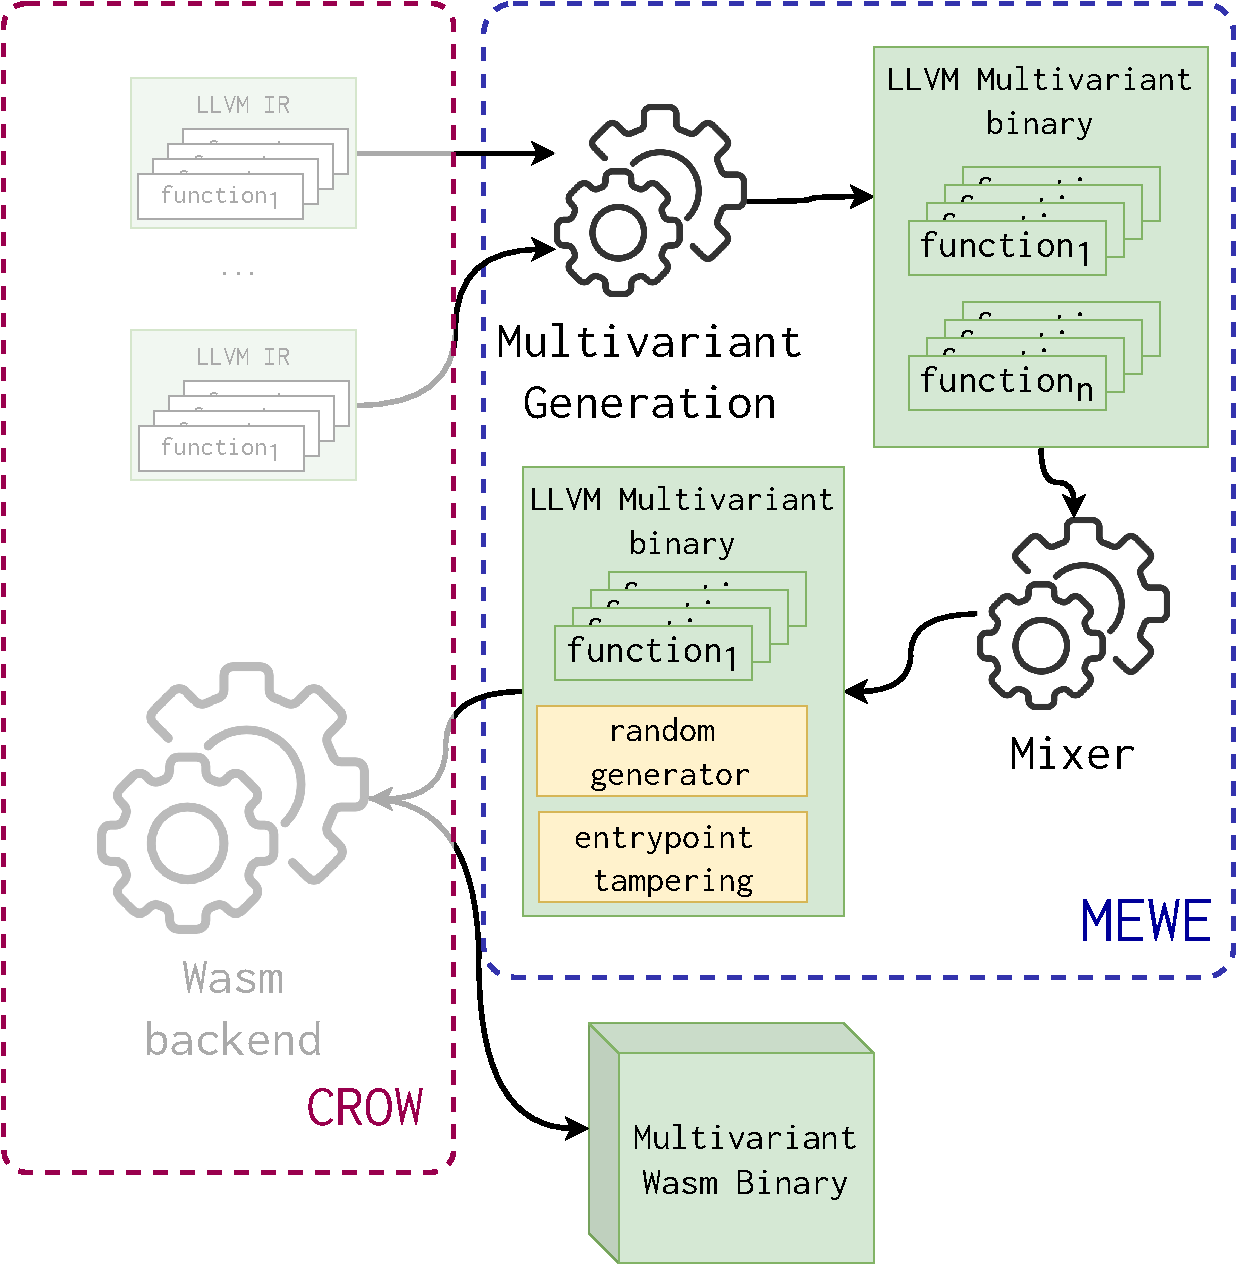
\includegraphics[height=3.2in]{diagrams/MEWE.pdf}
  \caption{Overview of \tool workflow. It takes as input an LLVM binary. It first generates a set of functionally equivalent variants for each function in the binary using CROW. Then, MEWE generates an LLVM multivariant binary composed of all the function variants. Finally, the Mixer includes the behavior in charge of selecting a variant when a function is invoked. Finally, the \tool mixer composes the LLVM multivariant binary with a random number generation library and tampers the original application entrypoint. The final process produces a \wasm\ multivariant binary ready to be deployed. }
  \label{workflow}
\end{figure*}


\msubsection{Multivariant generation}


The key component of \tool consists in combining the variants into a single binary.
The goal is to support execution-path randomization at runtime.
The core idea is to introduce one dispatcher function per original function with variants.
A dispatcher function is a synthetic function in charge of choosing a variant at random when the original function is called.
With the introduction of the dispatcher function,  \tool turns the original call graph into a multivariant call graph, defined as follows. 


\begin{figure}
    \centering
  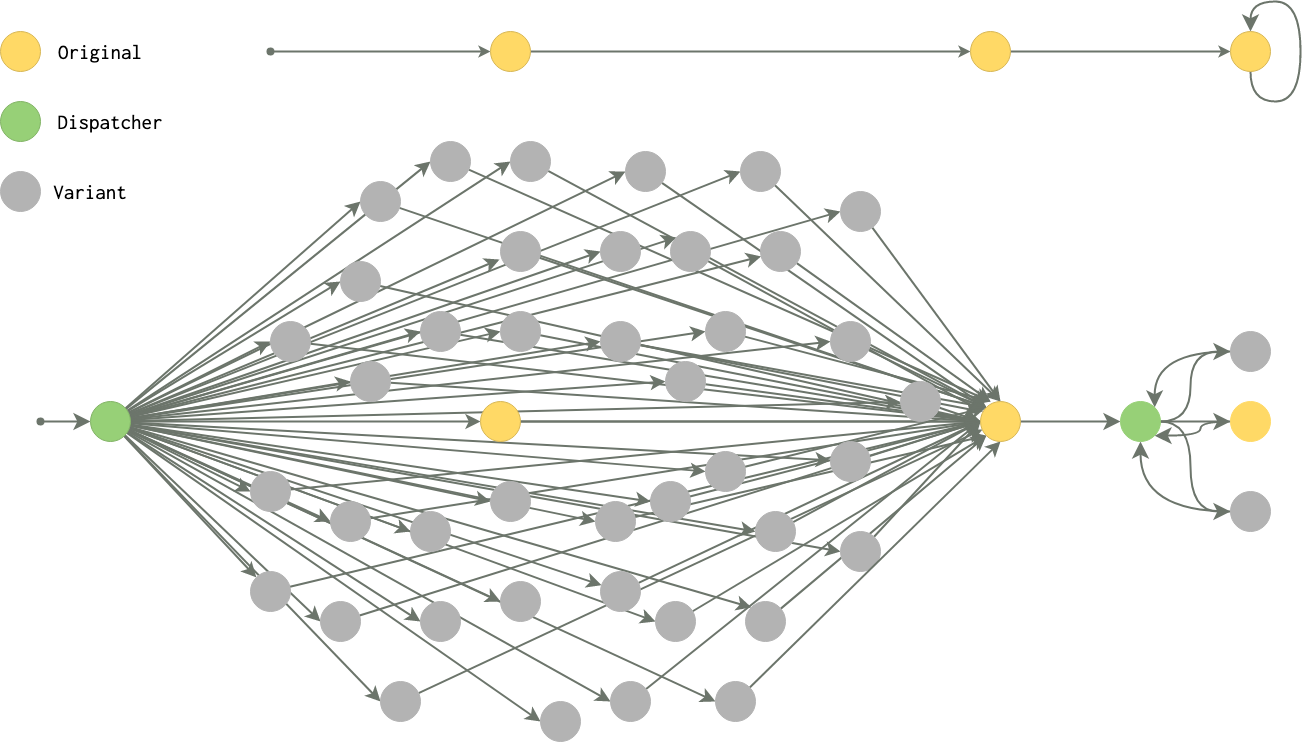
\includegraphics[width=.8\linewidth]{diagrams/CFG.png}
  \caption{Example of two static call graphs. At the top, the original call graph, at the bottom, the multivariant call graph, which includes nodes that represent function variants (in gray), dispatchers (in green), and original functions  (in yellow).
}
  \label{multivariant}
\end{figure}

% Instance of a multivariant module
In \autoref{multivariant}, we show the original static call graph for an original program (top of the figure), as well as the multivariant call graph generated with \tool (bottom of the figure).
The gray nodes represent function variants, the green nodes function dispatchers, and the yellow nodes are the original functions.
The directed edges represent the possible calls.
The original program includes three functions. \tool generates 43 variants for the first function, none for the second, and three for the third. 
\tool introduces two dispatcher nodes for the first and third functions. Each dispatcher is connected to the corresponding function variants to invoke one variant randomly at runtime.


% exaplanation of dispatcher
In  \autoref{listing:multivariant_template}, we illustrate the LLVM construction for the function dispatcher corresponding to the right most green node of \autoref{multivariant}.
It first calls the random generator, which returns a value used to invoke a specific function variant. 
We implement the dispatchers with a switch-case structure to avoid indirect calls that can be susceptible to speculative execution-based attacks \cite{Narayan2021Swivel}. 
The choice of a switch-case also avoids having multiple function definitions with the same signature, which could increase the attack surface in case the function signature is vulnerable \cite{johnson2021}.
This also allows \tool to inline function variants inside the dispatcher instead of defining them again.
Here we trade security over performance since dispatcher functions that perform indirect calls, instead of a switch-case,  could improve the performance of the dispatchers as indirect calls have constant time.
%It should be noted that the dispatcher function is constructed using the same signature as the original function. 


\lstset{
    language=llvm,
    %style=nccode,
    basicstyle=\footnotesize\ttfamily,
    columns=fullflexible,
    breaklines=true,
    numbers=none,
    stepnumber=1,
    float
}

\begin{code}
\scriptsize
\noindent\begin{minipage}[b]{\linewidth}
    \begin{minipage}[t]{1\linewidth}
        \begin{lstlisting}[escapeinside={(*}{*)}]
define internal i32 @foo(i32 %0) {
    entry:
      %1 = call i32 @discriminate(i32 3)
      switch i32 %1, label %end [
        i32 0, label %case_43_
        i32 1, label %case_44_
      ]
    case_43_:                 
      %2 = call i32 @foo_43_(%0)
      ret i32 %2
    case_44_:                
      %3 = <body of foo_44_ inlined>
      ret i32 %3
    end:                                             
      %4 = call i32 @foo_original(%0)
      ret i32 %4
}
        \end{lstlisting}
    \end{minipage}%
    
    \noindent\rule{\linewidth}{0.4pt}
    \captionof{lstlisting}{Dispatcher function embedded in the multivariant binary of the original function in the rightmost green node in \autoref{multivariant}.}\label{listing:multivariant_template}
\end{minipage}
\end{code}

\msubsection{The Mixer}

MEWE has four specific objectives: link the LLVM multivariant binary, inject a random generator, tamper the application's entrypoint, and merge all these components into a multivariant \wasm\ binary.
We use the Rustc compiler\footnote{\url{https://doc.rust-lang.org/rustc/what-is-rustc.html}} to orchestrate the mixing.
For the random generator, we rely on WASI's specification \cite{WASI} for the random behavior of the dispatchers. However, its exact implementation is dependent on the platform on which the binary is deployed.
The Mixer creates a new entrypoint for the binary called \emph{entrypoint tampering}.
It wraps the dispatcher for the entrypoint variants as a new function for the final Wasm binary and is declared as the application entrypoint. 

\msection{Wasm-mutate}

\todo{Motivate}
\todo{What happens with the other 30\% of the binaries?}

\msubsection{Variants' generation}

\todo{The egraph thingy}

\msection{Discussion}

\todo{Comparison of the approaches}


%\subsection{CROW}
%\todo{Do not mentioend superoptimizers. Talk in terms of SMT encoding.}

%\subsection{Constant inferring}

%\subsection{Disabling optimisations}

%\subsection{MEWE}


%\section{Approaches comparison}

%\section{Accompanying artifacts}